%% sigconf for double column
%% natbib for bibtex
%% nonacm because it is not for a conference
\documentclass[format=sigconf, natbib=true, nonacm=true]{acmart}
\usepackage{lipsum}
\usepackage{hyperref}
\begin{document}
    \title{Impact on End-users by ISP IPv6 Deployment}

    \author{Tim Niklas Gruel}
    \affiliation{
    \institution{Ruhr-Universität Bochum}
    \city{Bochum}
    \country{Germany}
    }
    \email{tim.gruel@rub.de}

    \begin{abstract}
        This paper presents an overview about different techniques to cope with the IPv4 address exhaustion. The impact on the end-users is on focus. First some early NAT based solutions are introduced. Later dualstack is discussed. At the end the IPv6 only solution, deployed by ISPs today, is presented. It turns out that the end-user, especially the technical experienced one, can experience great benefits with IPv6. With IPv6 the internet gets back to its routs. All devices can talk to each other and central server are not mandatory to establish communication.
    \end{abstract}

    \keywords{IPv6, Tunneling, Translation, End-user Impact, NAT64, DNS64, 464XLAT, Dualstack}

    %% page numbers
    \settopmatter{printfolios=true}

    \maketitle

    \section{INTRODUCTION}
    In the late 90s is became very clear, that the IPv4 address space is not sufficient to meet the future demand. The popularity of the Internet especially in the end-user marked was heavily underestimated at the creation of IPv4. There are approximately 4 billion IPv4 addresses. Today there are over 8 billion humans on earth. That means that two humans need to share a single IPv4 address, not considering servers. Today, a typical family has multiple devices per person, including TVs, gaming consoles, smart phones, personal computers and many more. This led to the assignment of the last available IPv4 block in the early 2010s. With the rise of smart home technology and IoT devices, the demand for IP addresses per houshould will not stop to incrise.In this paper I will present a nearly complete overview over the different idears to slow down the inevitable IPv4 exhaustion. Expect for the last one, none of these is a long term solution or even tries to solve the problem itself. ISPs tried to keep cost as low as possible. This led to keeping IPv4 addresses as long as possible.\\\\First, ISPs started to assign only one public IP per customer. The customer had to use NAT44 in order to provide all his end devices with an internet connection. The end-user was the one getting a worse experience. Over the time, assigning only one IPv4 per customer was too much for the ISPs. Especially with the rise of mobile internet and an even higher demand for addresses, IPv4 was doomed. ISPs tried to provide more IP addresses, by only assigning private IPv4s to customers, leading to NAT444. NAT itself has many problems, which will be discussed in this paper. NAT444 makes the problems even worse. End-users were and are still heavily effected by that.\\\\A few years later dualstack was provided by the ISPs. Dualstack introduced the next generation of IP addresses, called IPv6. Compared to IPv4 addresses which are a 32 Bit string, IPv6 addresses are a 128 Bit string. IPv6 solves the problem of address exhaustion completly. Unfortunately IPv6 is not backwards compatible to IPv4. Thus all infrastructure needs to be renewed. The Internet is fully decentralices. It is not possible to perform such a transition on one particular day. Dualstack implements both, IPv4 and IPv6. Devices and Servers supporting IPv6 can communicate over IPv6. In the case that one device is not yet capable of IPv6, IPv4 acts as a fallback. This is a perfect transition technology, but it is no solution for the IPv4 exhaustion problem. Each end-user still needs an public or private IPv4. The problem is not solved.\\\\Lately, ISP started to provide IPv6 only. This is also very common in mobile networks. The devices natively speak to servers over IPv6. For legacy IPv4 servers, there are different translation mechanisms. This paper will look deeper into NAT64 combined with DNS64. Moreover I will present 464XLAT and NAT-PT. All of are similar to a NAT44, but tranlating between IPv6 and IPv4. The interesting thing is, that these translation happens at the ISP, so the end-user only works with IPv6. This has many advantages for the end-user. Though, some legacy applications depending heavily on IPv4 cannot be used. One example for that is Skype.\\\\At the end of this paper, tunneling IPv6 in IPv4 and the other way around is presented. This happens only at ISP level, but indirectly influences the end-user to. Mainly in a better path availability, thus seemless internet service. There are many technologies, including 6in4, 6to4, 6over4, 6rd, Teredo, 4in6.\\\\In the last few years the apodption of IPv6 has increased rapidly. On \url{https://www.google.com/intl/en/ipv6/statistics.html} it is possible to view the current adoption of IPv6 regarding the Google landing page. Germany for example has an adoption of over 65\%. This statistics really shows the trend of ISPs worldwide, deploying IPv6 only or dualstack. Nearly all mobile clients use IPv6 today and are able to interact with the Internet without major notable disadvantages. Cisco predicts that the transition to IPv6 is finished in 2028. This means that nerly all end-users and servers world wide communicate over IPv6. That has great advantages for the end-user regarding security and opens up entirely new options for innovative peer to peer technologies. Hosting a Server on a smart phone might sound strange today, but could be a very usual thing in 10 years from now. The end-user is the one benefiting the most from unique, world-wide routable IP addresses.\\\\Now I am going to turn back the time a bit and we are focussing on the problem, emerging in the late 90s. It becomes clear that the IPv4 address space is not big enough. ISPs are searching for a solution. The main goal is to assign the same public, gloably routable IPv4 address to multiple devices. This is not meant for a long period of time, but much more as a quick fix, until the new standard IPv6 is developed.
    
    \section{EARLY SOLUTIONS}
    This section presents three different solution to to extend the lifetime of IPv4. I will discuss NAT44, A+P and NAT444. All these solutions aim to share one single IPv4 address between multiple end devices. It is important to understand theses technologies in order to correctly estimate the impact of IPv6 deployment by ISPs. Watching at modern solutions alone could leed to the impression, that these solutions are better or worse than they really are. Thus this paper starts at NAT44
    \subsection{NAT44}
    NAT44 is also kown as CPE NAT. The word NAT stands for \textit{Network Address Translation}. NAT44 means that one IPv4 address is translated to multiple IPv4 addresses. CPE means \textit{Customer Premise Equipment}. The whole NAT procedure is up to the end-user. The ISP only provides one single IPv4 address. Typically one public, globally routable IP is tranlated to multiple private IP addresses. There are three private IPv4 Blocks which are the following:
    \begin{enumerate}
        \item 10.0.0.0/8
        \item 172.16.0.0/12
        \item 192.168.0.0/16
    \end{enumerate}
    Everybody can use the IPv4 addresses in these blocks. Private IPv4 addresses will never be routed in the internet. Most end-users use the third option for their home network. Thus they can use 254 different devices which is sufficient for most users. All these 254 devices share one public IPv4. All of them share the $2^{16} = 65536$ ports of the public IPv4 too. From the outside you cannot decide whether only one device or multiple devices are behind the NAT. In the example \ref{fig:nat_44} is a NAT-Translation table. As you can see, the PC with IP \textit{192.168.0.10} cannot use all ports, because the PC with the IP \textit{192.168.0.12} uses the Port \textit{7035}. All ports are shared. This can lead to problems as we discuss later. NAT44 was the first solution to the IPv4 exhaustion problem. It is an easy fix, because the ISP has nothing to, except delivering one single IP per customer. Only the end-user needs a NAT compatible router.
    \begin{figure}
        \centering
        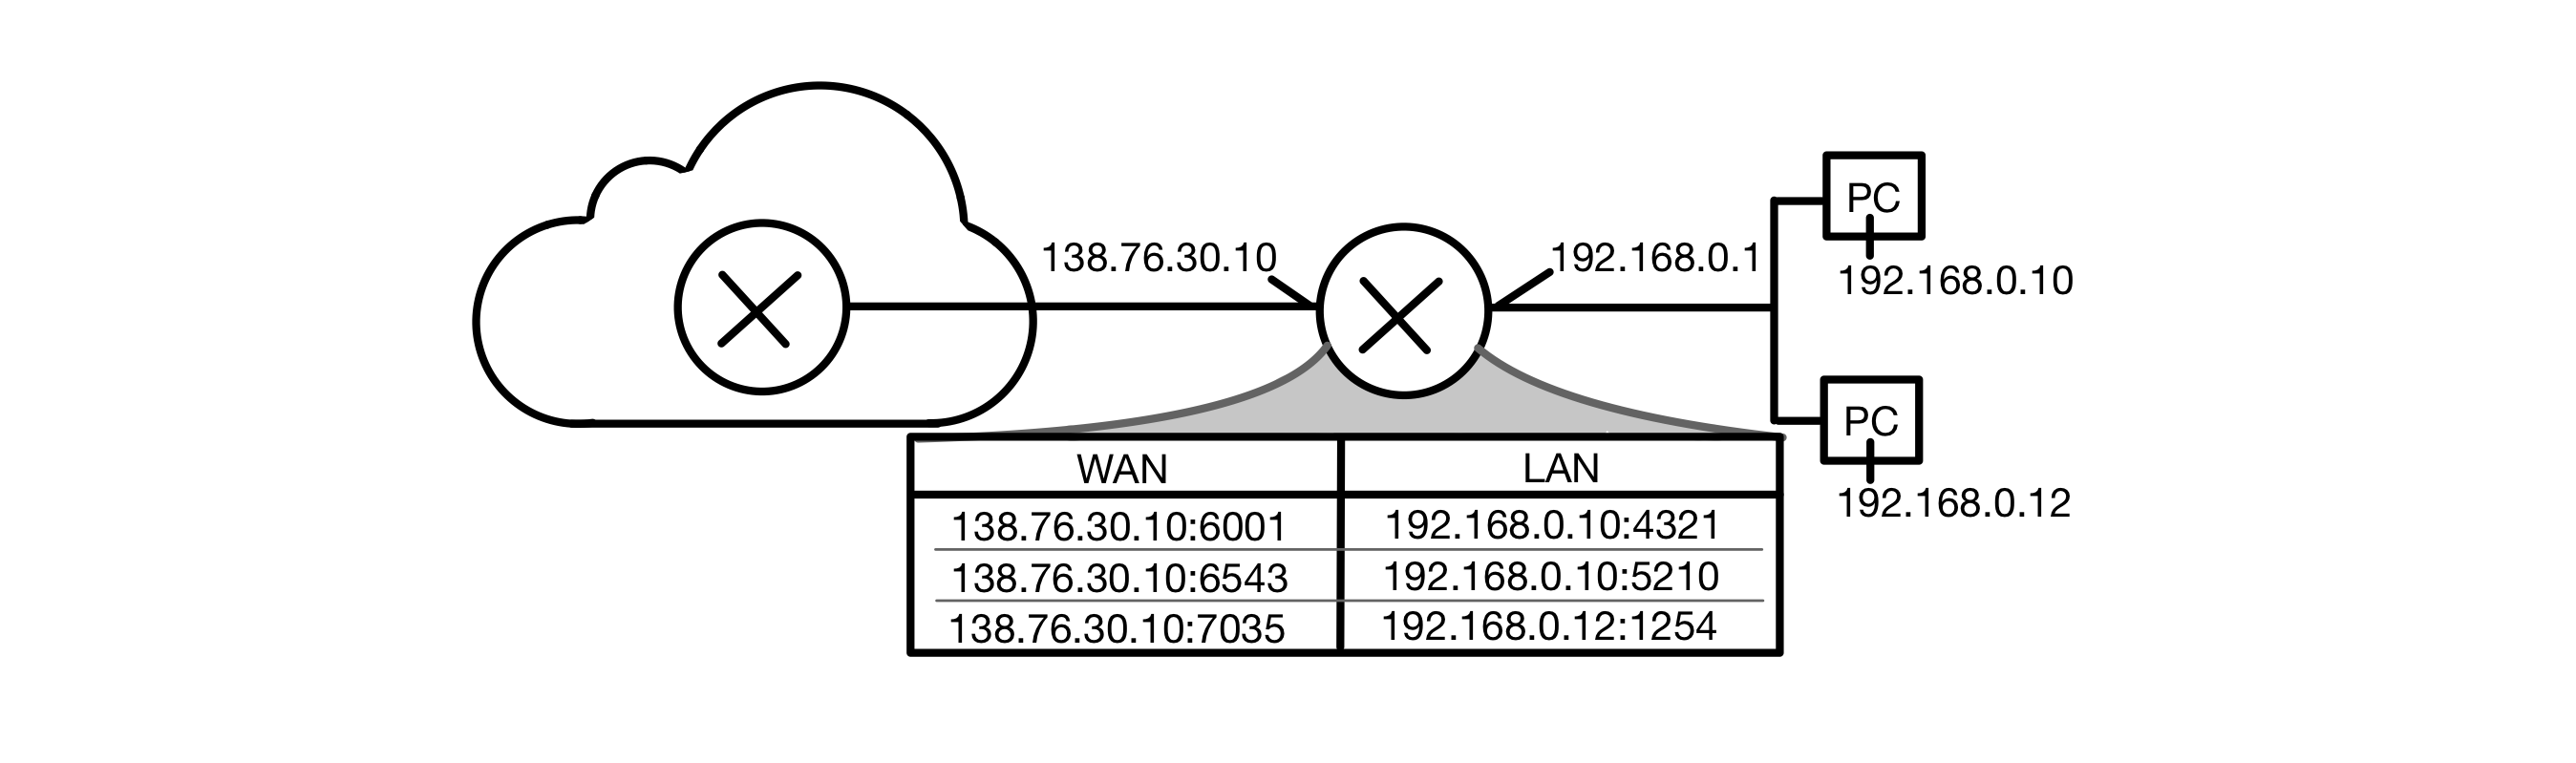
\includegraphics[width=0.4\textwidth]{images/nat_44.png}
        \caption{Example of NAT44 with NAT-Translation table}
        \label{fig:nat_44}
    \end{figure}

    \subsection{A+P}
    \lipsum[14-16]
    \subsection{NAT444}
    \lipsum[16-18]
    Smart author said you\cite{7119767} thta.
    \subsection*{END-USER IMPACT}
    \lipsum[18-22]

    \section{MODERN SOLUTIONS}
    \lipsum[21]
    \subsection{DUALSTACK}
    \lipsum[22-25]
    \subsection{DUALSTACK LITE}
    \lipsum[25-28]
    \subsection*{END-USER IMPACT}
    \lipsum[18-22]

    \section{LATEST SOLUTION: IPv6 ONLY}
    \lipsum[21]
    \subsection{TRANSLATION: NAT64/DNS64}
    \lipsum[22-24]
    \subsection{TRANSLATION: 464XLAT}
    \lipsum[24-26]
    \subsection{TRANSLATION: NAT-PT}
    \lipsum[26-28]
    \subsection*{END-USER IMPACT}
    \lipsum[18-21]

    \section{ISP Tunnels}
    \lipsum[21]
    \subsection{6in4}
    \lipsum[22-24]
    \subsection{4in6}
    \lipsum[24-26]
    \subsection{6to4}
    \lipsum[26-28]
    \subsection*{6over4}
    \lipsum[18-21]
    \subsection{6rd}
    \lipsum[26-28]
    \subsection*{Teredo}
    \lipsum[18-21]
    \subsection*{END-USER IMPACT}
    \lipsum[18-22]

    \section{Summary}
    \lipsum[100-104]

    %%section REFERENCES
    \bibliographystyle{plain}
    \bibliography{references}


\end{document}
